\clearpage
\section{Diffusion Distance}

The diffusion distance is given by $\sqrt{Dt}$, which is found in the equation that is used to describe the concentration after a time $t$ in a thin layer of the diffusing species is concentrated at $x=0$ of a semi-infinte sample \cite{diff}:
\begin{align}
  \label{eq:3}
  c(x,t)&=\dfrac{M}{\sqrt{\pi D t} \exp\left(-\dfrac{x^2}{4DT}\right)}.
\end{align}

The diffusion distance at room temperature was calculated for all systems. First, the diffusion coefficient at room temperature was calculated using equation \ref{eq:1} with the values of activation energy from table \ref{tab:tabla2}. The results are shown in the following table:

\begin{table}[H]
    \centering
    %\captionsetup{justification=centering}
    \begin{tabular}{ccccc}
        System & $D_0$ ($m^2/s$) & Q (kJ/mol) & $D_{278K}$ ($m^2/s$) \\ \hline \hline
        Ag-Ag & $2,70e-5$ & $182,96$ & $2,29e-37$ \\
        Al-Al & $1,37e-5$ & $124$ & $2,52e-27$ \\
        Cu-Cu & $1,05e-4$ & $210$ & $1,62e-41$ \\
        Ti-Ti & $3,4e-4$ & $328$ & $1,08e-61$ \\
        Ag-Cu & $3,10e-10$ & $72$ & $7,42e-23$ \\
        Ag-Pt & $1,30e-5$ & $258$ & $7,75e-51$ \\
        Ag-Ti & $1,00e-4$ & $279$ & $1,24e-53$ \\
        Al-Cu & $8,00e-6$ & $181$ & $1,50e-37$ \\
        Al-Pt & $1,30e-7$ & $194$ & $1,28e-41$ \\
        Al-Ti & $6,60e-3$ & $329$ & $1,41e-60$
    \end{tabular}
    \caption{Diffusion coefficient data calculated for room temperature ($278$ K)\\
    \textit{Source: Adapted from \citep{kakusan} database.}}
    \label{tab:tabla2}
\end{table}

With the diffusion coefficient calculated at toom temperature, the diffusion distance was calculated for all systems for time range from $0$ to $2e3$ seconds, using the expresion for diffusion distance from equation \ref{eq:3}

\subsection{Self-diffusion}

Distance as a fuction of time for self-diffusing systems is plotted in \ref{fig:self_x}. This plot, shows that for the aluminum self-diffusion system, the diffusion distance is higher than for the other self-diffusing systems. 

Because of the scales, it is difficult to properly see the behaviour of the distance for all systems, in order to observe the change of the diffusion distance with time the logarithmic scale is used. Figure \ref{fig:self_logx} shows the logarithm of the diuffusion distance as a function of the logarithm of time. In this graph the system of aluminum self-diffusion shows the highest diffusion didstance,meaning that the aluminum atoms move the farthes in the same time, which also corresponds to the higher diffusivity as it is shown on figure \ref{fig:self_lnd}, which corresponds to the low activation value of $124$ kJ/mol with respect to the activation energy values of the other systems.

On the other hand, the titanium self diffusion system has the lowest diffusion ditance, this also corresponds to this system having the highest activation energy as is obseverved in figure \ref{fig:self_lnd}, where this system has the steepest slope indicating that it requires more energy for the diffusion to occur, which also translates in a lower value for the distance that the atoms can move on the same period of time compared to a system that requires less energy for the diffusion to occur. 

\begin{figure}[h]
 \centering
 %\captionsetup{justification=centering}
  \subfloat[]{
   \label{fig:self_x}
    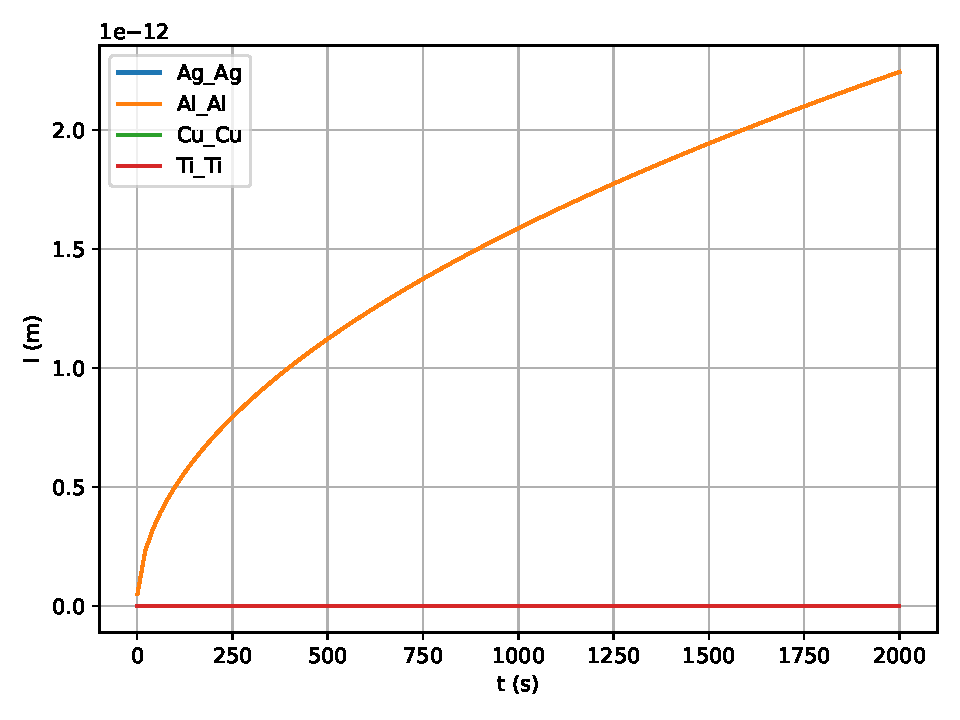
\includegraphics[width=0.5\textwidth]{graficas/l_self.pdf}}
  \subfloat[]{
   \label{fig:self_logx}
    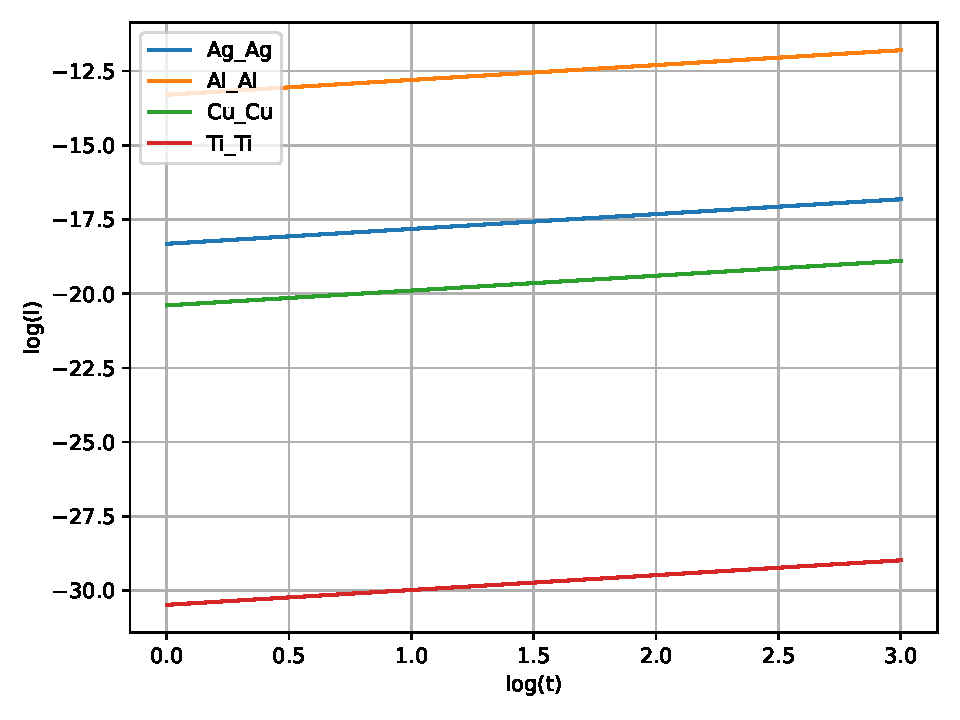
\includegraphics[width=0.5\textwidth]{graficas/log(l)_self.pdf}}
 \caption{a) Diffusion distance $l$ (m) as a function of time $t$ (s) and b) logarithm of the diffusion distance as a function of the logarithm of time for selft-diffusion systems. \\
 \textit{Source: Data from \citep{kakusan}, visualization by the author (code available at \citep{mygit}).}}
 \label{fig:self_length}
\end{figure}


\subsection{Solute diffusion}

Figure \ref{fig:length} presents the graphs for the diffusion distance for systems with aluminum and silver as solutes in copper, platinum and titanium. The plots in figure \ref{fig:x} show the diffusion distance as a function of time for all systems, where the system Ag-Cu (silver diffusing in copper) shows the highest diffusion distance than the other systems. The behaviour of all systems can be observed better in figure \ref{fig:logx}, where the logarithm of the diffusion distance is plotted as a funcion of the logarithm of time.

For the systems with silver as solute, figure \ref{fig:logx} shows that the highest distance is for the Ag-Cu silver, while the lowest distance is for the Ag-Ti system. This shows that silver atoms can diffuse a higher distance in copper than they can diffuse in platinum; which is consistent with the results obtained for the diffusion coefficient in figure \ref{fig:lnd}. It can also be seen that the diffusioin distancees for silver in platinum and titanium are in closer, which could be due to both metals having an hexagonal crystal structre; as well as having close values for activation energies: $258$ and $279$ kJ/mol for Ag-Pt and Ag-Ti respectively. 

For the systems where aluminum is a solute, from figure \ref{fig:logx}, it can be seen that the Al-Cu systems has the highest diffusion distance, as a contrast with Al-Pt and Al-Ti systems.  Which indicates that aluminum can diffuse more easily in copper than in platinum or titanium. It can also be seen that systems Al-Cu and Al-Pt have closer values of diffusion distance, even though the crystal structures for copper and platinum are different, they do have close values of activation energy, $181$ and $194$ kJ/mol for Al-Cu and Al-Pt respectively. In the case of the Al-Ti system, the diffusion distance is the lowest, which corresponds to the higher value of activation energy for this systeem ($329$ kJ/mol), meaning that it requires more energy for the aluminum atoms to diffuse in titanium than it does for diffusion in copper and platinum.  

\begin{figure}[h]
 \centering
 %\captionsetup{justification=centering}
  \subfloat[]{
   \label{fig:x}
    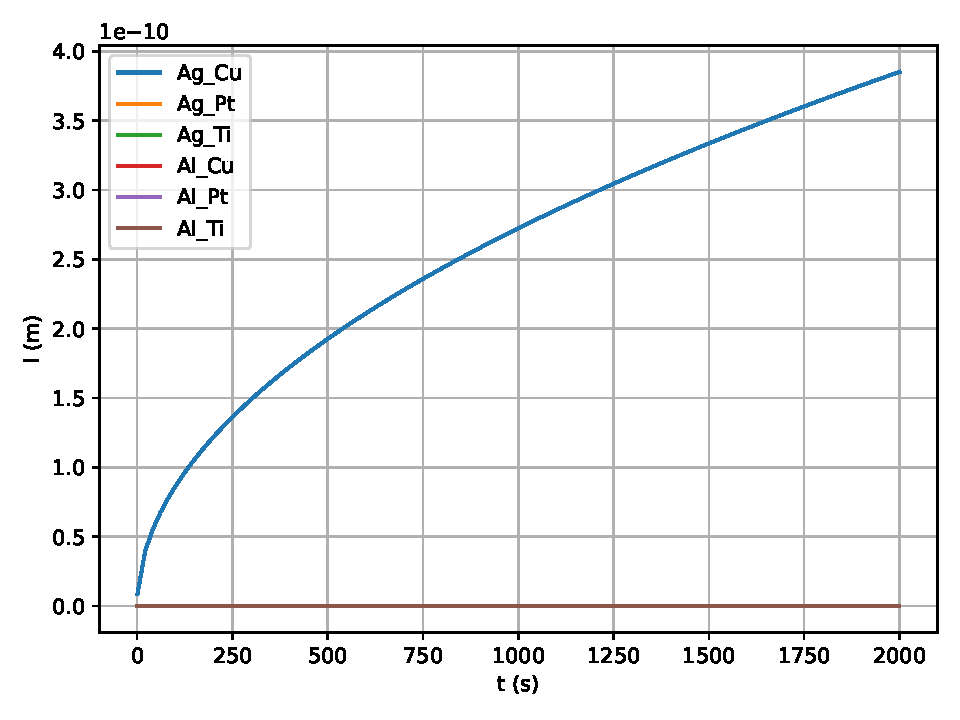
\includegraphics[width=0.5\textwidth]{graficas/l_other.pdf}}
  \subfloat[]{
   \label{fig:logx}
    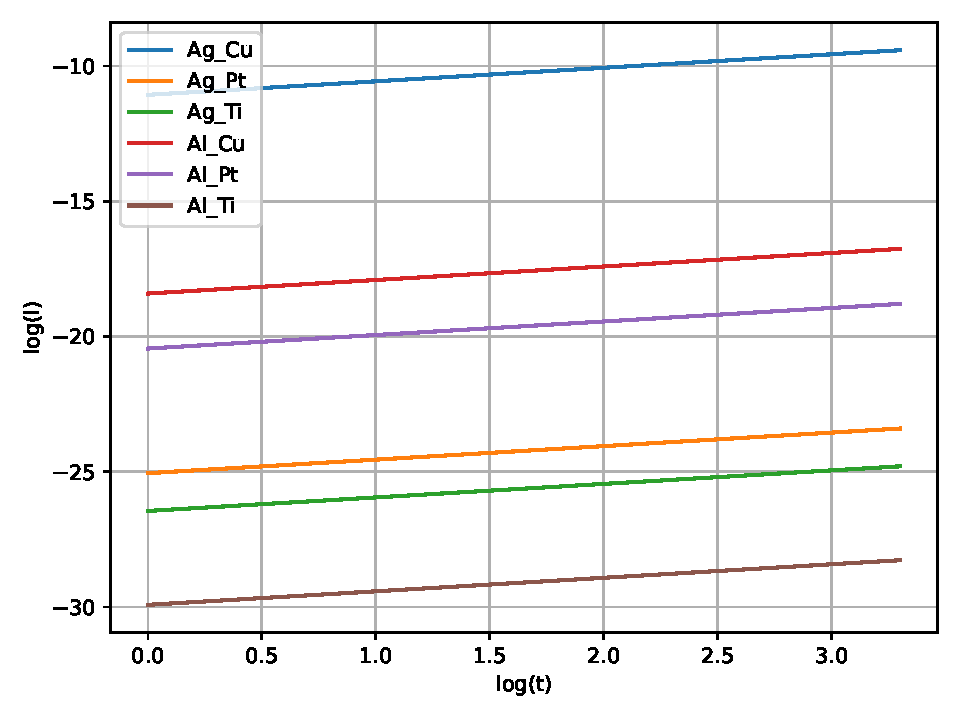
\includegraphics[width=0.5\textwidth]{graficas/log(l)_other.pdf}}
 \caption{a) Diffusion distance $l$ (m) as a function of time $t$ (s) and b) logarithm of the diffusion distance as a function of the logarithm of time. \\
 \textit{Source: Data from \citep{kakusan}, visualization by the author (code available at \citep{mygit}).}}
 \label{fig:length}
\end{figure}



%How far atoms have diffused in a given time.

%The rate of atomic motion in each material.

%Observations:
%Ag_Ag shows the highest diffusion length → silver atoms move the farthest in the same time → highest self-diffusivity.

%Ti_Ti shows the lowest diffusion length → titanium atoms diffuse more slowly.

%The curves are non-linear (parabolic), reflecting the square-root time dependence from the formula above.